\section{Date: 2026-07-25}
\noindent \textbf{Series ID: Y055RC1A027NBEA} 

\noindent This series is titled Government Gross Investment: Intellectual Property Products and has a frequency of Annual. The units are Billions of Dollars and the seasonal adjustment is Not Seasonally Adjusted.The observation start date is 1929-01-01 and the observation end date is 2025-01-01.The popularity of this series is 1. \\ 

\noindent \textbf{Series ID: CIS1013000000000I} 

\noindent This series is titled Employment Cost Index: Total compensation for All Civilian workers in Manufacturing and has a frequency of Quarterly. The units are Index Dec 2005=100 and the seasonal adjustment is Seasonally Adjusted.The observation start date is 2003-01-01 and the observation end date is 2026-01-01.The popularity of this series is 2. \\ 

\subsection{Raw Regression}
\noindent Regresses the two series against each other directly. A significant result here can come just as easily from both series sharing a long-run trend as from any real relationship.

\begin{center}
\begin{tabular}{lclc}
\toprule
\textbf{Dep. Variable:}               & value\_fred\_CIS1013000000000I & \textbf{  R-squared:         } &     0.958   \\
\textbf{Model:}                       &              OLS               & \textbf{  Adj. R-squared:    } &     0.956   \\
\textbf{Method:}                      &         Least Squares          & \textbf{  F-statistic:       } &     484.1   \\
\textbf{Date:}                        &        Sat, 25 Jul 2026        & \textbf{  Prob (F-statistic):} &  5.52e-16   \\
\textbf{Time:}                        &            12:55:27            & \textbf{  Log-Likelihood:    } &   -65.151   \\
\textbf{No. Observations:}            &                 23             & \textbf{  AIC:               } &     134.3   \\
\textbf{Df Residuals:}                &                 21             & \textbf{  BIC:               } &     136.6   \\
\textbf{Df Model:}                    &                  1             & \textbf{                     } &             \\
\textbf{Covariance Type:}             &           nonrobust            & \textbf{                     } &             \\
\bottomrule
\end{tabular}
\begin{tabular}{lcccccc}
                                      & \textbf{coef} & \textbf{std err} & \textbf{t} & \textbf{P$> |$t$|$} & \textbf{[0.025} & \textbf{0.975]}  \\
\midrule
\textbf{const}                        &      57.3163  &        3.046     &    18.816  &         0.000        &       50.981    &       63.651     \\
\textbf{value\_fred\_Y055RC1A027NBEA} &       0.2886  &        0.013     &    22.003  &         0.000        &        0.261    &        0.316     \\
\bottomrule
\end{tabular}
\begin{tabular}{lclc}
\textbf{Omnibus:}       &  4.531 & \textbf{  Durbin-Watson:     } &    0.215  \\
\textbf{Prob(Omnibus):} &  0.104 & \textbf{  Jarque-Bera (JB):  } &    2.139  \\
\textbf{Skew:}          &  0.450 & \textbf{  Prob(JB):          } &    0.343  \\
\textbf{Kurtosis:}      &  1.808 & \textbf{  Cond. No.          } &     788.  \\
\bottomrule
\end{tabular}
%\caption{OLS Regression Results}
\end{center}

Notes: \newline
 [1] Standard Errors assume that the covariance matrix of the errors is correctly specified.

\begin{figure}
\centering
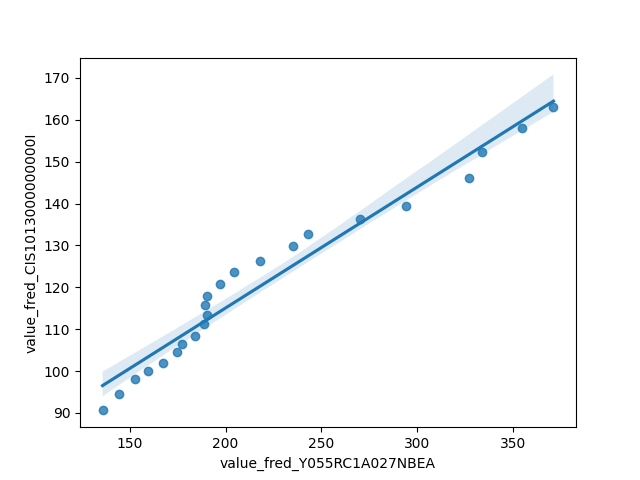
\includegraphics[scale = 0.9]{plots/plot_2026-07-25.png}
\caption{Raw Regression Plot for 2026-07-25}
\end{figure}
\newpage
\subsection{Detrended Regression}
\noindent Regresses the residuals of each series after removing its own linear time trend, so a shared trend can no longer drive the result on its own. A relationship that stays significant here is better evidence of a genuine link between the two series.

\begin{center}
\begin{tabular}{lclc}
\toprule
\textbf{Dep. Variable:}                          & value\_fred\_CIS1013000000000I\_detrended & \textbf{  R-squared:         } &     0.842   \\
\textbf{Model:}                                  &                    OLS                    & \textbf{  Adj. R-squared:    } &     0.835   \\
\textbf{Method:}                                 &               Least Squares               & \textbf{  F-statistic:       } &     112.3   \\
\textbf{Date:}                                   &              Sat, 25 Jul 2026             & \textbf{  Prob (F-statistic):} &  6.97e-10   \\
\textbf{Time:}                                   &                  12:55:27                 & \textbf{  Log-Likelihood:    } &   -40.429   \\
\textbf{No. Observations:}                       &                       23                  & \textbf{  AIC:               } &     84.86   \\
\textbf{Df Residuals:}                           &                       21                  & \textbf{  BIC:               } &     87.13   \\
\textbf{Df Model:}                               &                        1                  & \textbf{                     } &             \\
\textbf{Covariance Type:}                        &                 nonrobust                 & \textbf{                     } &             \\
\bottomrule
\end{tabular}
\begin{tabular}{lcccccc}
                                                 & \textbf{coef} & \textbf{std err} & \textbf{t} & \textbf{P$> |$t$|$} & \textbf{[0.025} & \textbf{0.975]}  \\
\midrule
\textbf{const}                                   &    5.629e-12  &        0.306     &  1.84e-11  &         1.000        &       -0.637    &        0.637     \\
\textbf{value\_fred\_Y055RC1A027NBEA\_detrended} &       0.1364  &        0.013     &    10.595  &         0.000        &        0.110    &        0.163     \\
\bottomrule
\end{tabular}
\begin{tabular}{lclc}
\textbf{Omnibus:}       &  3.828 & \textbf{  Durbin-Watson:     } &    0.613  \\
\textbf{Prob(Omnibus):} &  0.147 & \textbf{  Jarque-Bera (JB):  } &    2.028  \\
\textbf{Skew:}          & -0.611 & \textbf{  Prob(JB):          } &    0.363  \\
\textbf{Kurtosis:}      &  3.790 & \textbf{  Cond. No.          } &     23.8  \\
\bottomrule
\end{tabular}
%\caption{OLS Regression Results}
\end{center}

Notes: \newline
 [1] Standard Errors assume that the covariance matrix of the errors is correctly specified.

\begin{figure}
\centering
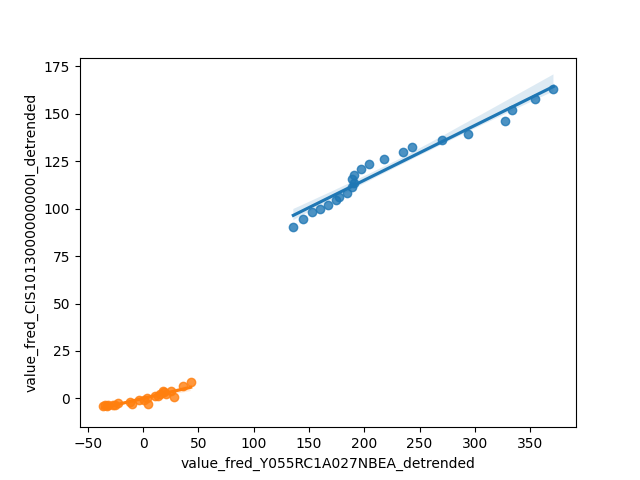
\includegraphics[scale = 0.9]{plots/plot_2026-07-25_detrended.png}
\caption{Detrended Regression Plot for 2026-07-25}
\end{figure}
\newpage
